% Algebra 2 Lesson 2-1 Lesson Quiz, short form (from the 2024 TE Lesson Quiz block, a2_2-1_TE.tex,
% checked against aga_24_a2_na_0201_lq.pdf). The form keeps the Savvas item numbers: items 3, 4, 5 (the
% items the kept Examples 4 and 5 teach; re-cut 2026-10-31 toward the Topic 2 test). Savvas items 1 and 2
% are left off (see the key).
\documentclass[11pt]{article}
\usepackage[margin=0.7in]{geometry}
\usepackage{amsmath,amssymb}
\usepackage{enumitem}
\usepackage{tikz}
\usepackage{pgfplots}
\pgfplotsset{compat=1.18}
\usepackage{fancyhdr}
\usepackage{parskip}
\setlist[enumerate]{leftmargin=*, itemsep=6pt}
\pagestyle{fancy}
\fancyhf{}
\fancyfoot[L]{\small\textit{en}Vision\textsuperscript{\textregistered} Algebra 2}
\fancyfoot[C]{\small 2-1 Lesson Quiz, short form}
\fancyfoot[R]{\small\thepage}
\renewcommand{\headrulewidth}{0pt}
\newcommand{\choice}[1]{\tikz[baseline=-0.6ex]\node[draw, circle, inner sep=0.6pt, minimum size=3.3mm, font=\scriptsize\bfseries] {#1};\;}
\newcommand{\checkbox}{$\square$\;}
\pgfplotsset{quizgrid/.style={
  axis lines=middle, grid=both, grid style={gray!45},
  ticklabel style={font=\scriptsize, fill=white, inner sep=1pt},
  xlabel={$x$}, ylabel={$y$}, axis line style={thick}, clip=true}}

\begin{document}

\noindent\textbf{Name}\; \rule{6cm}{0.4pt} \hfill Period \rule{1.2cm}{0.4pt} \quad Date \rule{2.2cm}{0.4pt}

\vspace{4pt}\noindent\rule{\textwidth}{0.6pt}

\vspace{2pt}\noindent{\LARGE\textbf{2-1 \; Lesson Quiz: Vertex Form of a Quadratic Function}}

\vspace{4pt}\noindent\rule{\textwidth}{0.6pt}

\vspace{6pt}
\textbf{3.} What is the equation written in vertex form of a parabola with a vertex of $(9,-1)$ that passes through $(7,7)$?

\vspace{4pt}
\begin{minipage}[t]{0.40\textwidth}
\begin{itemize}[leftmargin=1.2em, itemsep=5pt]
\item[] \choice{A} $y=2(x-9)^2-1$
\item[] \choice{B} $y=2(x+1)^2-9$
\item[] \choice{C} $y=2(x-7)^2+7$
\item[] \choice{D} $y=7(x-9)^2-1$
\end{itemize}
\end{minipage}\hfill
\begin{minipage}[t]{0.56\textwidth}
Show how you found $a$.

\vspace{4pt}
$y=a(x-\rule{0.8cm}{0.4pt})^2+\rule{0.8cm}{0.4pt}$

\vspace{12pt}\rule{\linewidth}{0.4pt}

\vspace{12pt}\rule{\linewidth}{0.4pt}
\end{minipage}

\vspace{10pt}\noindent\rule{\textwidth}{0.4pt}

\vspace{6pt}
\begin{minipage}[t]{0.56\textwidth}
\textbf{4.} Which of the following is an equation in the form \mbox{$y=ax^2+bx+c$} of the parabola shown in the graph?

\vspace{4pt}
\begin{itemize}[leftmargin=1.2em, itemsep=5pt]
\item[] \choice{A} $y=-5x^2-20x-65$
\item[] \choice{B} $y=-5x^2-20x-20$
\item[] \choice{C} $y=-x^2-27x-90$
\item[] \choice{D} $y=-5x^2+20x+25$
\end{itemize}

\vspace{6pt}
From the graph: vertex $(\rule{1cm}{0.4pt},\rule{1cm}{0.4pt})$ \quad $y$-intercept \rule{1.2cm}{0.4pt}

\vspace{6pt}
Show how you found $a$:

\vspace{12pt}\rule{\linewidth}{0.4pt}

\vspace{12pt}\rule{\linewidth}{0.4pt}
\end{minipage}\hfill
\begin{minipage}[t]{0.40\textwidth}
\vspace{-4pt}
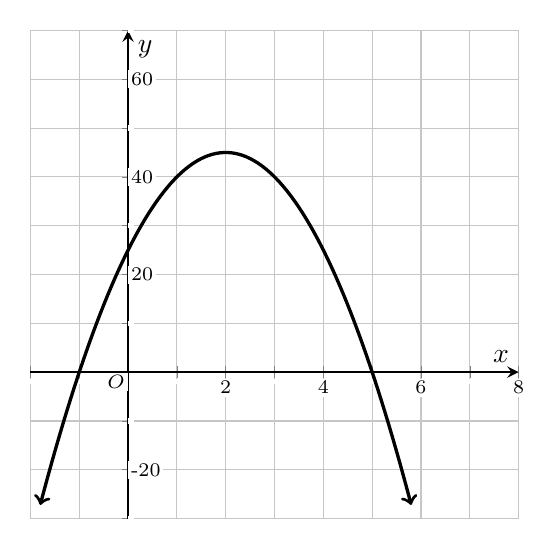
\begin{tikzpicture}
\begin{axis}[quizgrid, xmin=-2, xmax=8, ymin=-30, ymax=70,
  xtick={-2,...,8}, xticklabels={,,,,2,,4,,6,,8},
  ytick={-30,-20,...,70}, yticklabels={,-20,,,,20,,40,,60,},
  yticklabel style={anchor=west, xshift=2pt},
  x=0.62cm, y=0.062cm]
\addplot[very thick, domain=-1.8:5.8, samples=100, <->] {-5*(x-2)^2+45};
\node[font=\scriptsize, fill=white, inner sep=1pt, anchor=north east] at (axis cs:0,0) {$O$};
\end{axis}
\end{tikzpicture}
\end{minipage}

\vspace{10pt}\noindent\rule{\textwidth}{0.4pt}

\vspace{6pt}
\textbf{5.} Function $g$ is a transformation of the parent function $f(x)=x^2$. The graph of $g$ is a translation right 3 units and down 5 units of the graph of $f$. What is the equation of function $g$ written in the form $y=ax^2+bx+c$?

\vspace{4pt}
\begin{tabular}{@{}p{0.22\textwidth}p{0.22\textwidth}p{0.22\textwidth}p{0.22\textwidth}@{}}
\choice{A} $y=x^2+6x+4$ & \choice{B} $y=x^2-6x+4$ & \choice{C} $y=x^2+10x+22$ & \choice{D} $y=x^2-6x+14$
\end{tabular}

\vspace{6pt}
Show your work. Vertex form first: $g(x)=\rule{3.5cm}{0.4pt}$ \quad Then expand:

\vspace{12pt}\rule{\linewidth}{0.4pt}

\vspace{12pt}\rule{\linewidth}{0.4pt}

\vfill
\noindent\textbf{Scoring:} Question 4 and Question 5 are 10 points each. Question 3 is a bonus of up to 5 points. Total out of 20. (Questions 1 and 2 of the Savvas quiz are not on this form.)

\newpage
\noindent{\LARGE\textbf{2-1 Lesson Quiz, short form: answer key}}

\vspace{4pt}\noindent\rule{\textwidth}{0.6pt}

\begin{enumerate}
\item[\textbf{3.}] \textbf{A, $y=2(x-9)^2-1$.} $y=a(x-9)^2-1$; substitute $(7,7)$: $7=a(7-9)^2-1$, $8=4a$, $a=2$. Distractor C puts the point where the vertex goes; D uses the point's $y$ for $a$. DOK 2, skill F60. Taught by Example 4 steps 1--3 (Example 3 is the same substitution; cut). Topic 2 test item 1 (the golf ball) is this move in context. \textbf{Bonus 5:} 5 for A with the substitution shown; 3 for A with no work.
\item[\textbf{4.}] \textbf{D, $y=-5x^2+20x+25$.} From the graph the vertex is $(2,45)$ and the $y$-intercept is $25$. $25=a(0-2)^2+45$, $-20=4a$, $a=-5$. $y=-5(x-2)^2+45=-5(x^2-4x+4)+45=-5x^2+20x+25$. Check: $c=25$ is the $y$-intercept; the zeros $x=-1$ and $x=5$ match the graph. DOK 2, skill F16. Taught by Example 4 (Try It 4). \textbf{10 points:} 6 for D, 2 for the vertex and $y$-intercept read correctly, 2 for $a=-5$ shown.
\item[\textbf{5.}] \textbf{B, $y=x^2-6x+4$.} Right 3 and down 5 move the vertex to $(3,-5)$, and a translation keeps $a=1$: $g(x)=(x-3)^2-5=x^2-6x+9-5=x^2-6x+4$. Distractor A uses $(x+3)^2$ (left 3); C uses $(x+5)^2-3$ (the 3 and 5 swapped); D uses $(x-3)^2+5$ (up 5). DOK 2, skills F16, F68. Taught by Example 5 (Try It 5a). Topic 2 test item 2 is this move after a reflection in the $x$-axis. \textbf{10 points:} 6 for B, 2 for the vertex form $g(x)=(x-3)^2-5$, 2 for the expansion shown.
\end{enumerate}

\textbf{Items left off this form} (available for a retake or Form B): Savvas item 1, select all true statements about $g(x)=(x+2)^2+4$ as a transformation of $f(x)=x^2$ (answer B, C; DOK 2, F60 and F68; Example 1, cut); Savvas item 2, $h(x)=-\frac{1}{2}(x-4)^2+3$ is a bird's height, which point is the greatest height (answer A, $(4,3)$; DOK 2, F60; Example 2, cut).

\textbf{IXL replacement:} SmartScore 70 or above on URV and KQL replaces this quiz with 20/20.

\end{document}
